\documentclass[letterpaper,12pt,]{article}

\usepackage{titling}

\setlength{\droptitle}{5in}   % This is your set screw

\usepackage[%
    left=1in,%
    right=1in,%
    top=1in,%
    bottom=1.0in,%
    paperheight=11in,%
    paperwidth=8.5in%
]{geometry}%
\usepackage{comment}

\usepackage{listings}
\usepackage{graphicx}
\usepackage{amsmath}
\usepackage[section]{placeins}
\usepackage[font=small,skip=-2pt]{caption}
\usepackage{subcaption}
\usepackage{hyperref}
\usepackage{booktabs}
\usepackage{pdfpages}


\lstdefinestyle{mystyle}{
    %backgroundcolor=\color{backcolour},   
    %commentstyle=\color{codegreen},
    %keywordstyle=\color{magenta},
    %numberstyle=\tiny\color{codegray},
    %stringstyle=\color{codepurple},
    basicstyle=\footnotesize,
    breakatwhitespace=false,         
    breaklines=true,                 
    captionpos=b,                    
    keepspaces=true,                 
    numbers=left,                    
    numberstyle=\footnotesize,               
    stepnumber=1,
    numbersep=5pt,
    showspaces=false,                
    showstringspaces=false,
    showtabs=false,                  
    tabsize=2,
    frame=single
}
\lstset{frame=single}

\pagestyle{empty} % Remove page numbering
\linespread{1.5} % Line Spacing

\begin{document}

\begin{titlepage}

\newcommand{\HRule}{\rule{\linewidth}{0.5mm}} % Defines a new command for the horizontal lines, change thickness here

\center % Center everything on the page
 
%----------------------------------------------------------------------------------------
%	HEADING SECTIONS
%----------------------------------------------------------------------------------------


\textsc{\LARGE McGill University}\\[3.5cm]
\textsc{\Large Computational Aerodynamics}\\[0.5cm] 
\textsc{\large MECH 539}\\[2.5cm]

%----------------------------------------------------------------------------------------
%	TITLE SECTION
%----------------------------------------------------------------------------------------

{ \huge \bfseries Project 2}\\[1.5cm] % Title of your document

\HRule \\[0.4cm]
%----------------------------------------------------------------------------------------
%	AUTHOR SECTION
%----------------------------------------------------------------------------------------

\begin{minipage}{0.4\textwidth}
\begin{flushleft} \large
\emph{Name:}\\
Doug \textsc{Shi-Dong} % Your name
\end{flushleft}
\end{minipage}
~
\begin{minipage}{0.4\textwidth}
\begin{flushright} \large
\emph{Student ID:} \\
260466662\\
\end{flushright}
\end{minipage}\\[4cm]

\vfill{}
{\large February 18, 2016}\\[2cm]

\end{titlepage}


\section*{Question 1 \& 2}

The hand-written derivation is given on the last page.
The truncation error of the second-order finite-difference discretization is $\mathcal{O}((\Delta x)^2, (\Delta y)^2\ $) as expected. 
The modified equation in this case is simply the PDE on the LHS and the truncation error on the RHS.
The truncation error only contains even terms, therefore the error is purely dissipative.


\section*{Question 3}

Figure \ref{fig:u400} shows the solution for a $400 \times 400$ grid.

\begin{figure}[!h]
    \centering
    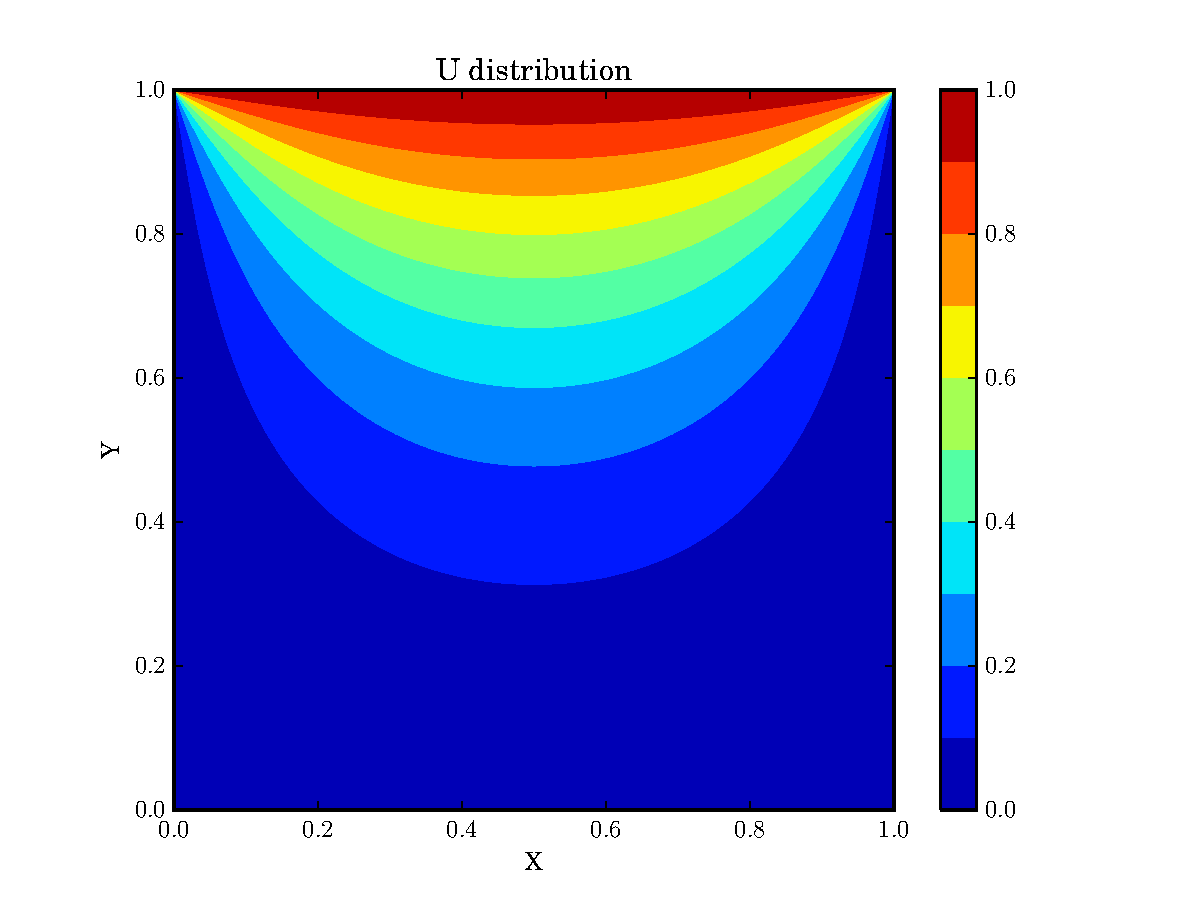
\includegraphics[width = 0.95\textwidth]{./Figures/U400.pdf}
    \caption{Numerical Solution $nx = 400$}
    \label{fig:u400}
\end{figure}


\newpage
\section*{Question 4}

The convergence plots over the iterations are shown in Figure \ref{fig:conv100}-\ref{fig:conv400}.
The convergence criterion is the maximum change in the solution $max(\Delta u) < 1\textsc{E-}6$.
The relaxation factor of the Successive Over-Relaxation (SOR) method is 1.5.

From the figures, it is obvious that Jacobi requires the most iterations, followed by Gauss-Seidel and then SOR. As the grid size increases, more iterations are required in order to converge to the same tolerance.

The Forsythe-Moler method is used to approximate the condition number of the A matrix since direct inversion would be too costly.
Both the numerical solution of the Laplace equation and the linear system from the Forsythe-Moler are evaluated until $max(\Delta u) < 1\textsc{E-}15$ is reached.
SOR is used to due its fast convergence.
The condition number is compiled in Table \ref{tab1}.
The condition number increases with grid size. It is consistent with the fact that bigger grid sizes require more iterations to converge.
\begin{table}[h]
\centering
\begin{tabular}{cccc} \toprule
    {Grid Size} & {100} & {200} & {400}\\ \midrule
    {Condition Number} & 1968 & 7905  & 29028\\
\bottomrule
\end{tabular}
\caption{Condition Number for Various Grid Sizes}
\label{tab1}
\end{table}


\begin{figure}[!h]
    \centering
    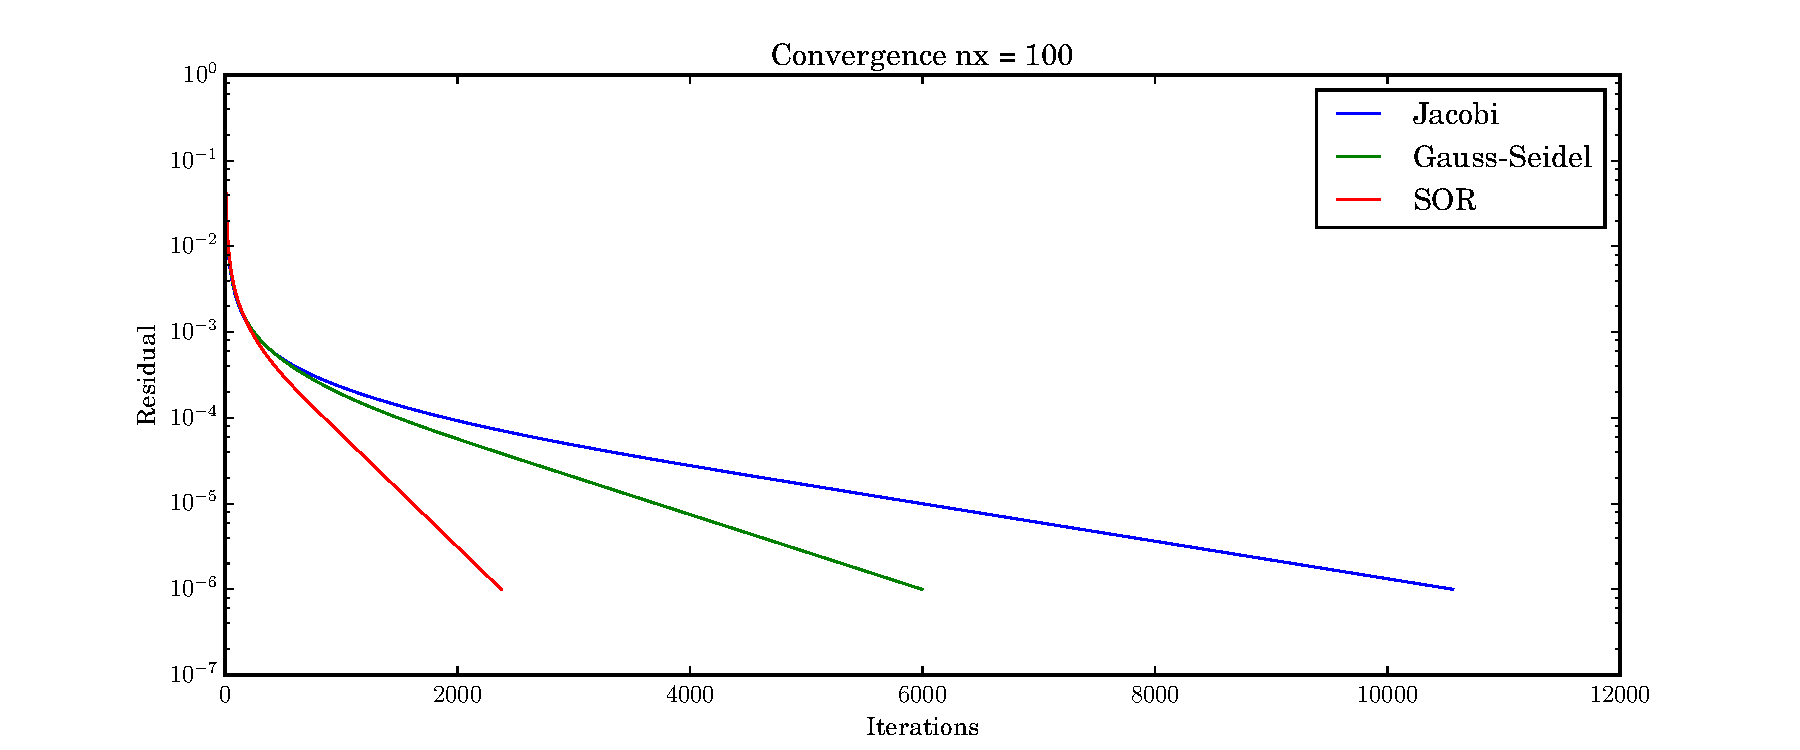
\includegraphics[width = 0.85\textwidth]{./Figures/Conv100.pdf}
    \caption{Convergence over Iterations $nx = 100$}
    \label{fig:conv100}
\end{figure}

\begin{figure}[!h]
    \centering
    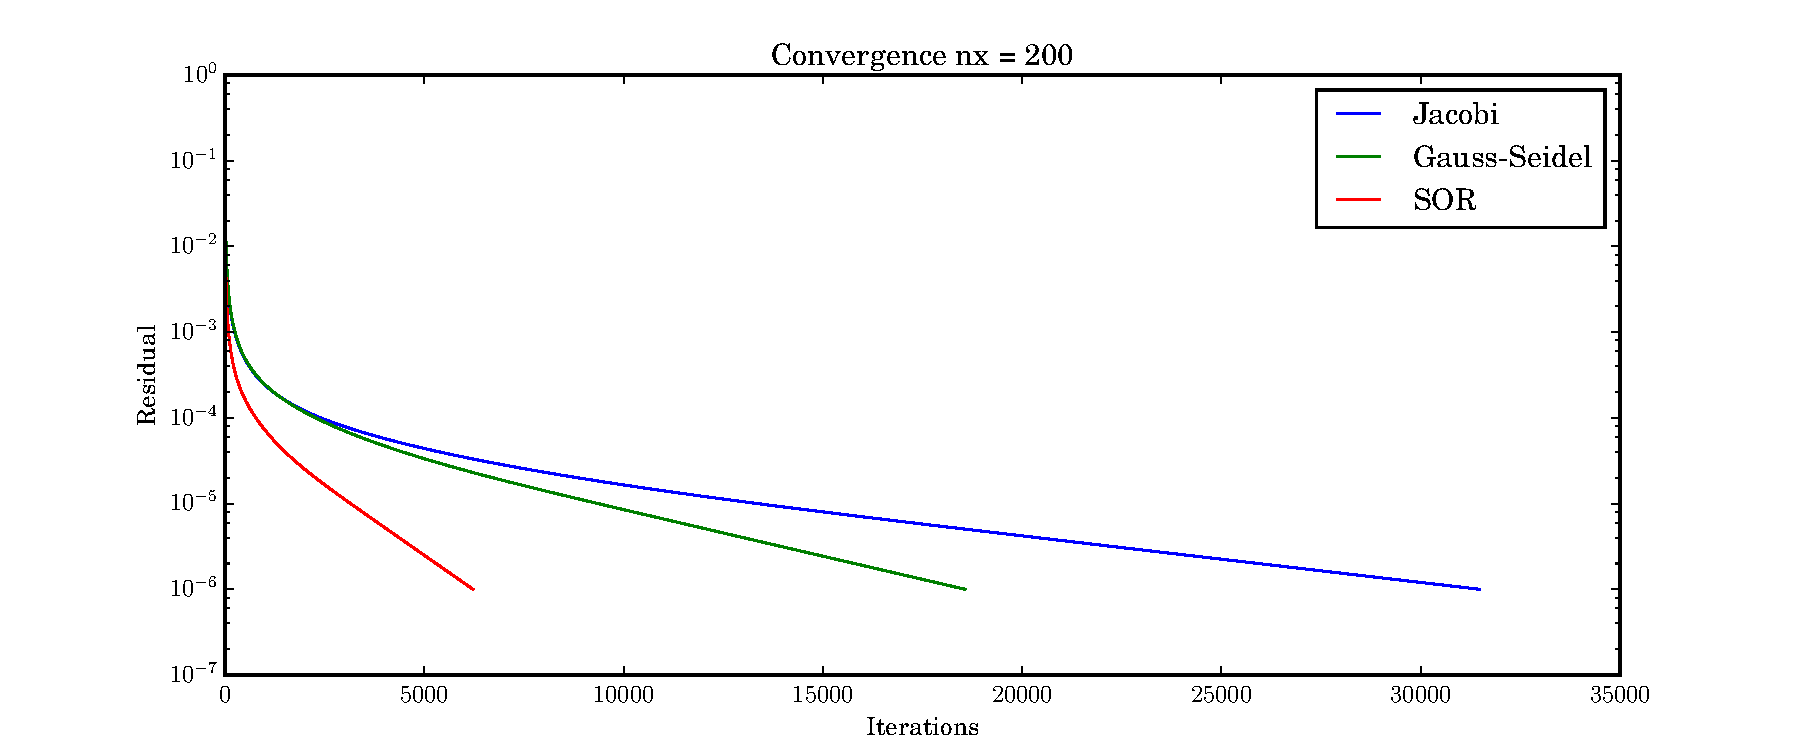
\includegraphics[width = 0.85\textwidth]{./Figures/Conv200.pdf}
    \caption{Convergence over Iterations $nx = 200$}
    \label{fig:conv200}
\end{figure}
\begin{figure}[!h]
    \centering
    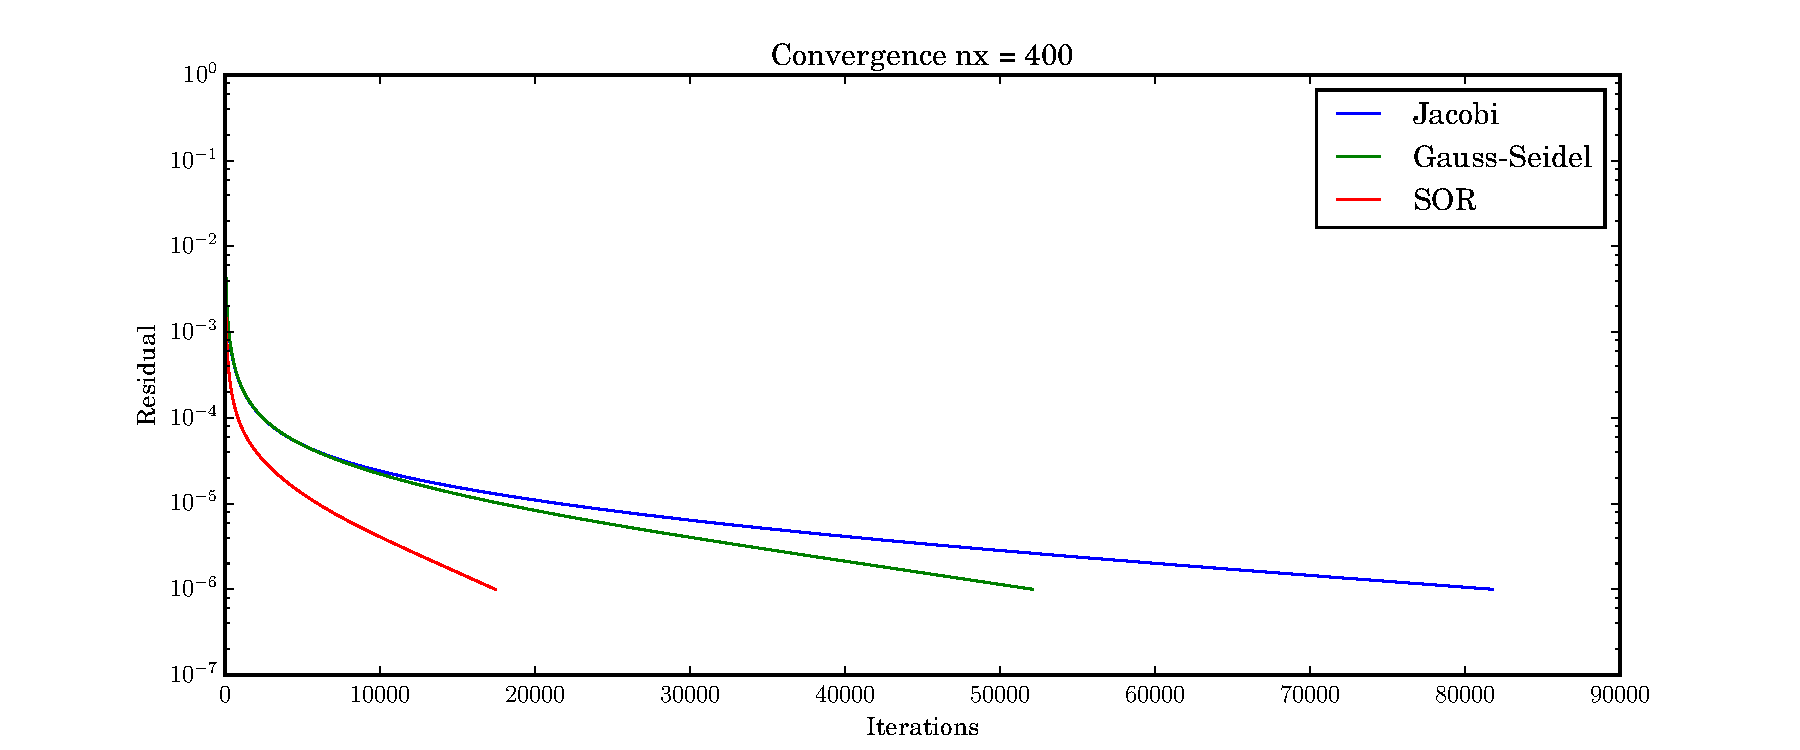
\includegraphics[width = 0.85\textwidth]{./Figures/Conv400.pdf}
    \caption{Convergence over Iterations $nx = 400$}
    \label{fig:conv400}
\end{figure}
\section*{Question 5}

The convergence of the residual versus CPU time is shown in Figure \ref{fig:time100}-\ref{fig:time400}. Note that the computation has been done in FORTRAN with optimization level -O3.

SOR still dominates the other two methods in terms of performance.
However, the difference between Gauss-Seidel and Jacobi has reduced considerably. 
Although Jacobi takes almost twice as many iterations, the CPU time is close to Gauss-Seidel. 
Therefore, each iteration of Jacobi is less costly.

Table \ref{tab2} compiles results to compare time and iterations for the different schemes for $nx = 400$ with the debugging flag (-g) and with optimization flag (-O3).
Jacobi keeps the previous solution $k$ in memory while it is computing $k+1$, therefore it requires twice as much memory as Gauss-Seidel or SOR.
Although it is more costly in terms of memory, it allows for a few improvements in terms of speed.
First, the dependence of the previous iteration allows the problem to be divided into parallel problems, allowing parallel computation.
Second, the compiler is aware that the $k+1$ step is only dependent on the $k$ step, therefore, it is able to better optimize the process in terms of accessing memory.

It can be seen that in debug mode, the iteration of each method is approximately the same cost in terms of CPU time.
However, Jacobi is much faster than the other two methods when -O3 is enabled due to the simplicity of memory access. SOR is the slowest per iteration since it requires more complicated memory accesses.

\begin{table}[h]
\centering
\begin{tabular}{cccc} \toprule
    {} & {Jacobi} & {Gauss-Seidel} & {SOR}\\ \midrule
    {Iterations} & 81787 & 52109 & 23340\\
    {Time (O3)} & 48.96 & 45.68 & 28.23\\
    {Time/Iterations (O3)} & 0.599 & 0.877 & 1.210\\
    {Time (g)} & 429.09 & 265.84 & 125.07\\
    {Time/Iterations(g)} & 5.24 & 5.10 & 5.36\\
\bottomrule
\end{tabular}
\caption{Time and Iterations for Different Methods $nx = 400$}
\label{tab2}
\end{table}

\begin{figure}[!h]
    \centering
    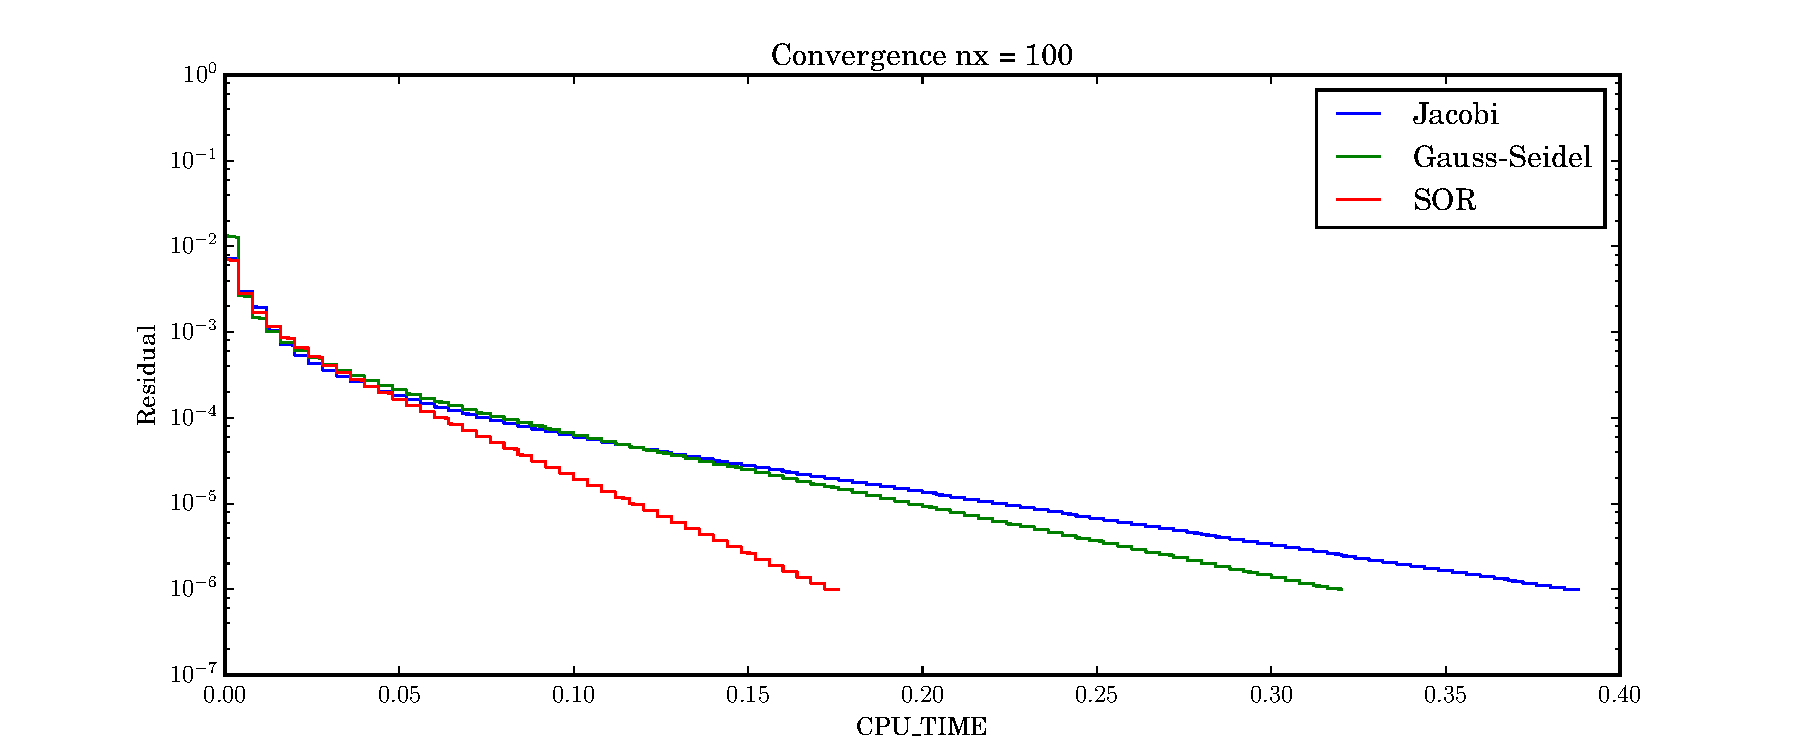
\includegraphics[width = 0.85\textwidth]{./Figures/time100.pdf}
    \caption{Convergence over Time $nx = 100$}
    \label{fig:time100}
\end{figure}

\begin{figure}[!h]
    \centering
    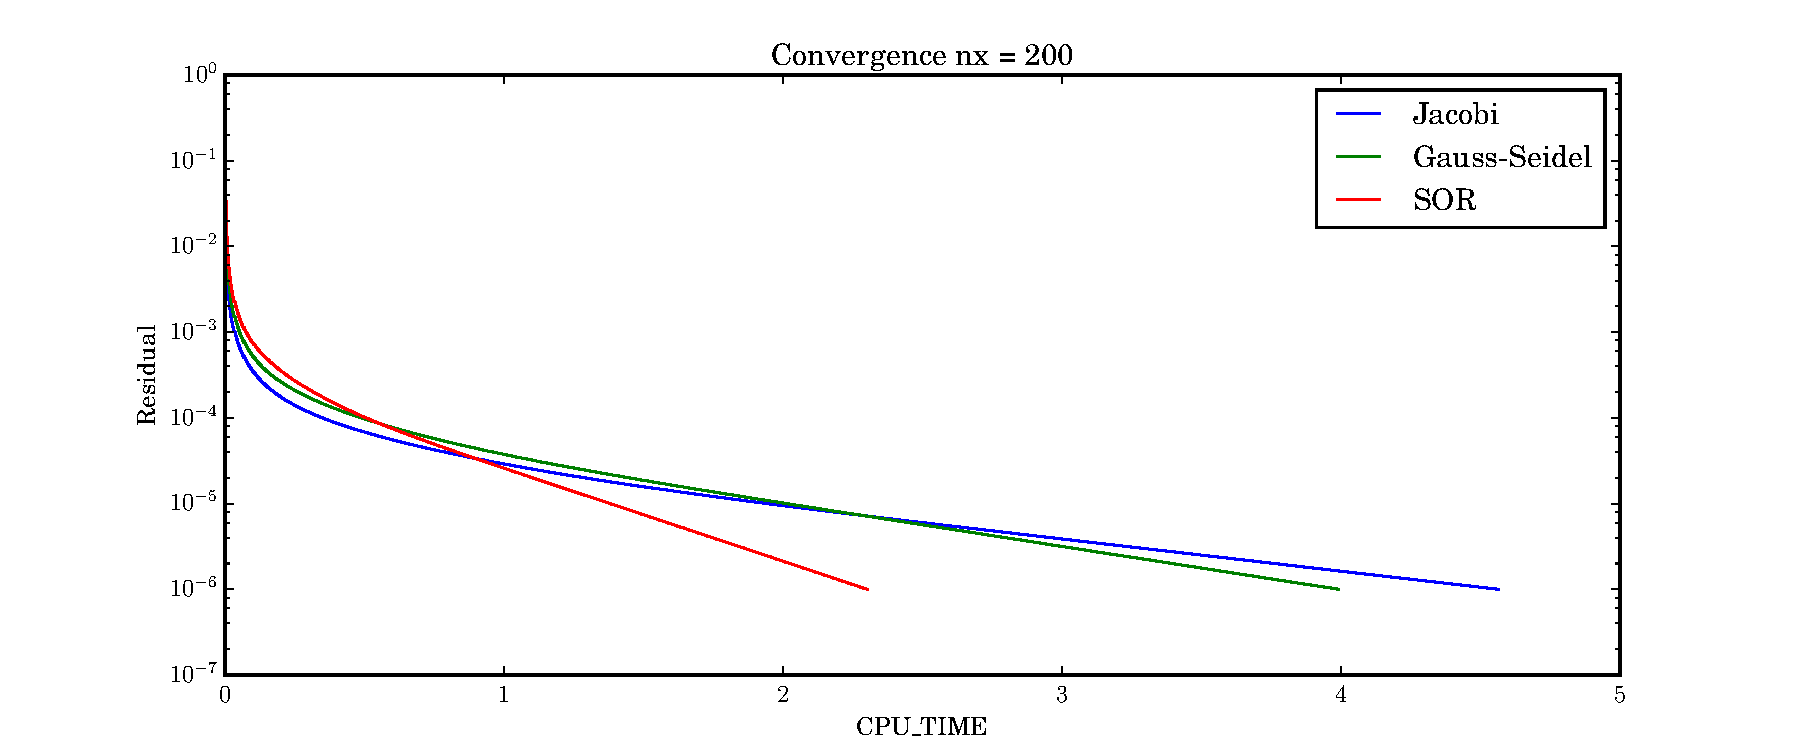
\includegraphics[width = 0.85\textwidth]{./Figures/time200.pdf}
    \caption{Convergence over Time $nx = 200$}
    \label{fig:time200}
\end{figure}
\begin{figure}[!h]
    \centering
    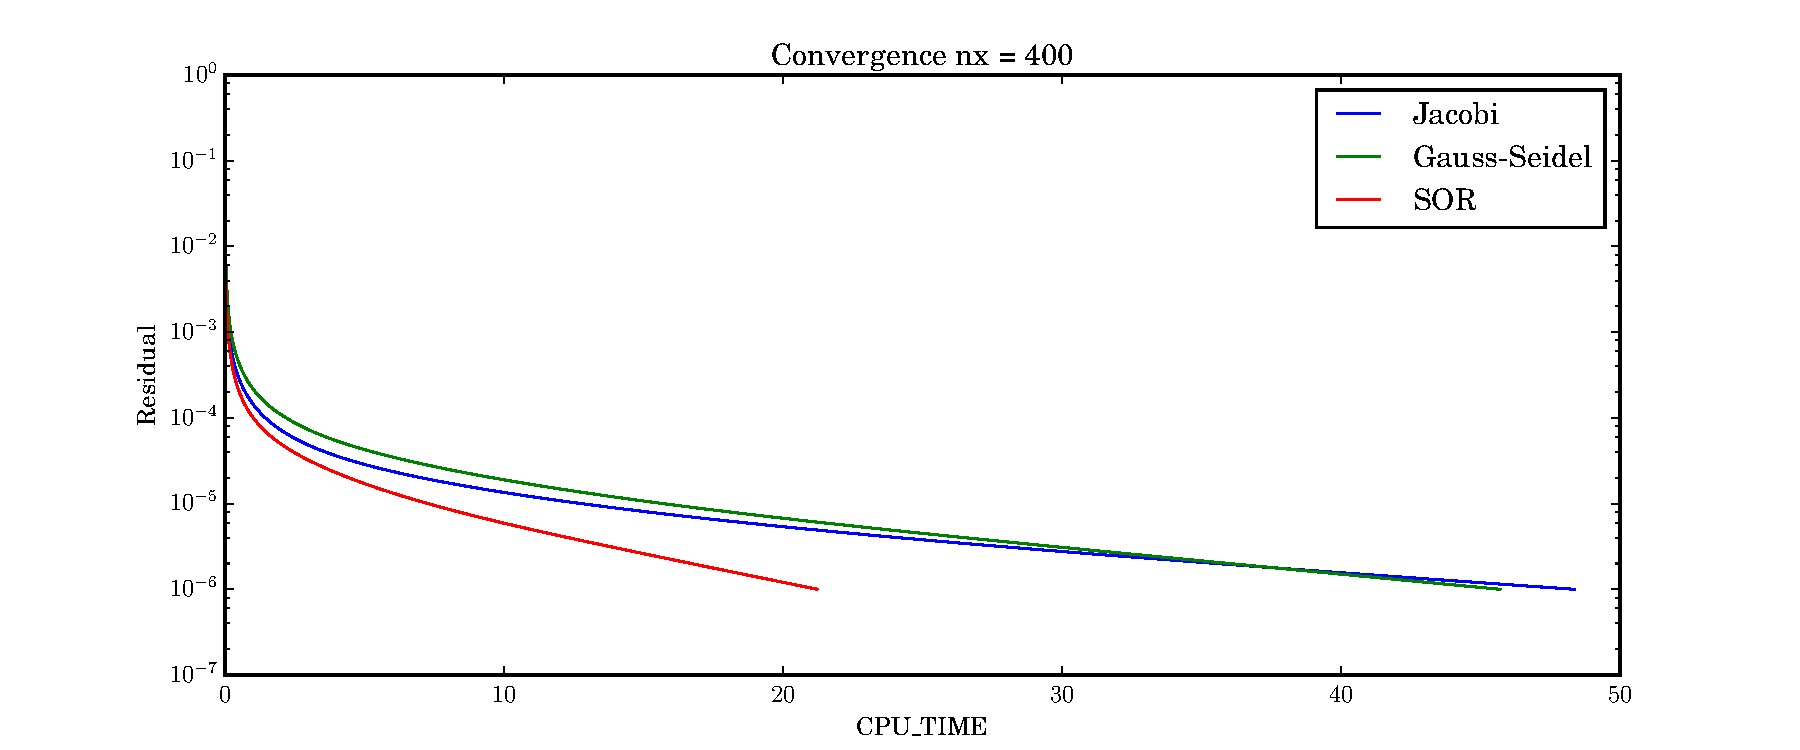
\includegraphics[width = 0.85\textwidth]{./Figures/time400.pdf}
    \caption{Convergence over Time $nx = 400$}
    \label{fig:time400}
\end{figure}

\section*{Question 6}

The exact solution is given by Equation \ref{eq1}.
Numerically, 3600 terms have been used to evaluate the exact solution.
However, the exact solution sum cannot resolve the straight line boundary accurately.
Only 3 to 4 digits are recovered.
Therefore, the exact solution itself contains some error near the boundaries.

\begin{equation}
\begin{split}
U(x,y) = \sum^{\infty}_{n=1} c_n sinh(n\pi y) sin(n \pi x)\\
c_n = 2 \int_0^1 sin(n \pi x) dx / sinh(n\pi)
\end{split}
\label{eq1}
\end{equation}

The absolute error of the numerical solution versus the approximated analytical solution is show in Figure \ref{fig:errorc}. Along
For this reason, the relative error is calculated using the L1-norm due to its robustness against outliers.
Figure \ref{fig:error} shows the error versus the grid size.
First, all iterative methods give the same error as it would be expected since the same linear system is being solved.
Second, the logarithmic slope is nearly 2, meaning that the error is proportial to $(\Delta x)^2$, which corresponds to second-order accuracy.


\begin{figure}[!h]
    \centering
    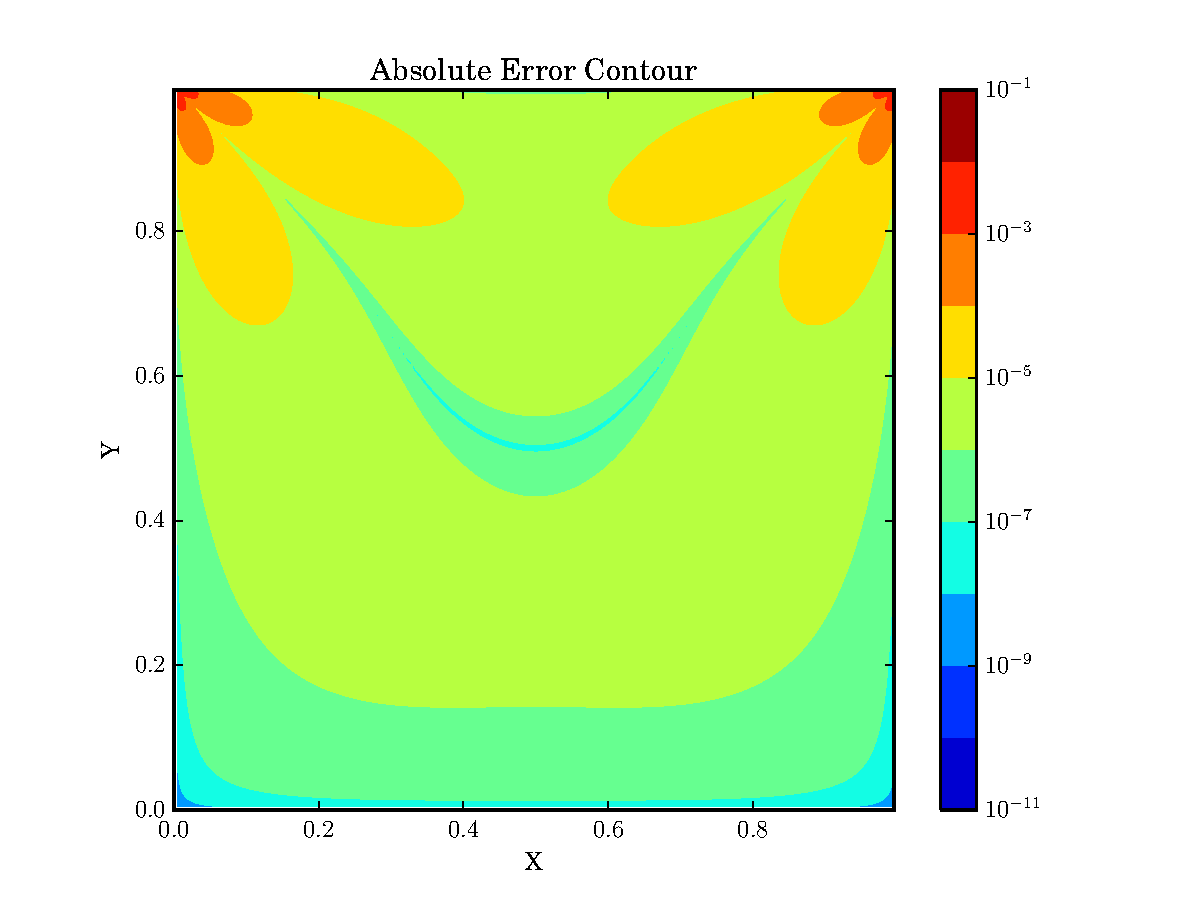
\includegraphics[width = 0.65\textwidth]{./Figures/ErrorContour.pdf}
    \caption{Contour Plot of Absolute Error}
    \label{fig:errorc}
\end{figure}

\begin{figure}[!h]
    \centering
    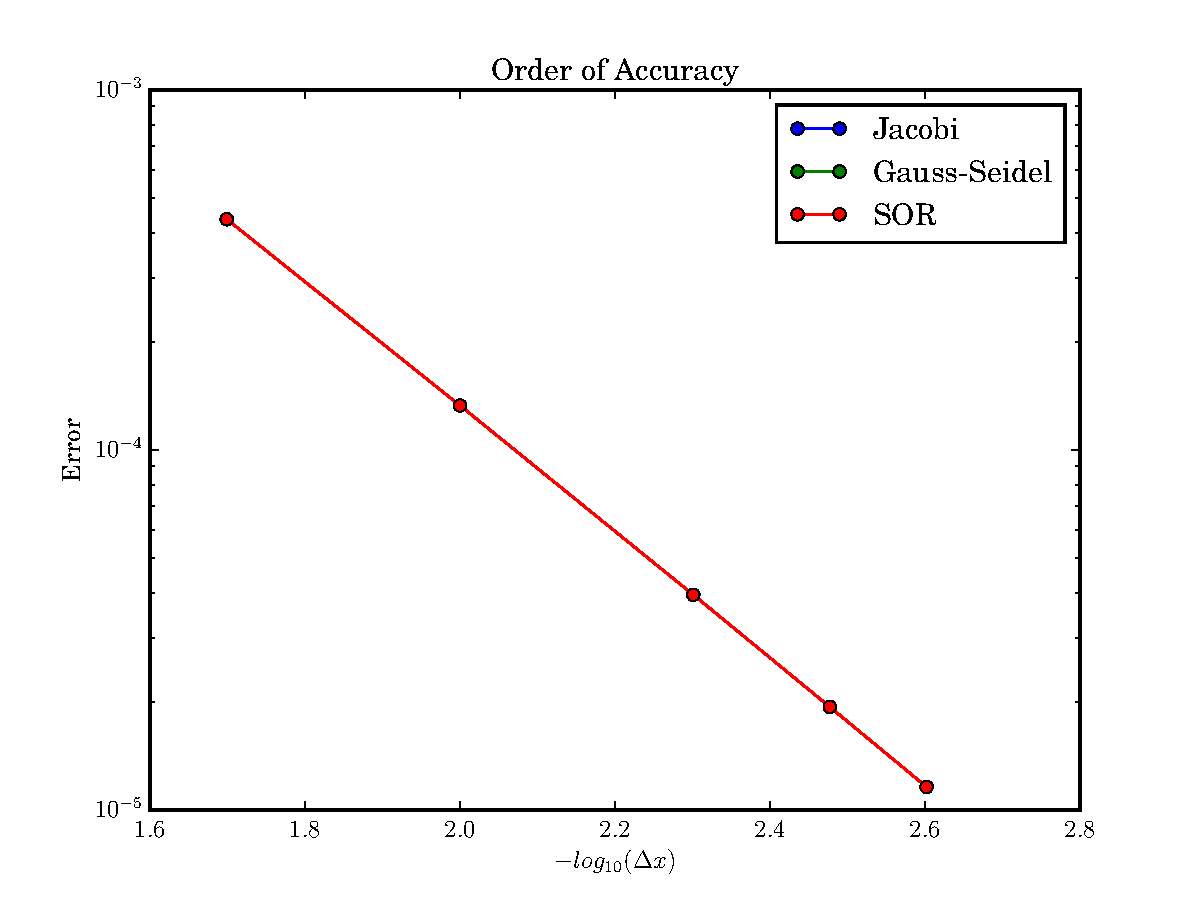
\includegraphics[width = 0.65\textwidth]{./Figures/Error.pdf}
    \caption{Order of Accuracy}
    \label{fig:error}
\end{figure}


\section*{Question 7}

Figure \ref{fig:sor100}-\ref{fig:sor400} show the convergence of the SOR method for different relaxation parameters and grid sizes.
When the relaxation parameter is less than 1, it takes more iterations than GS.
When it is exactly 1, the exact GS is retrieved.
For values above 1, increasing the relaxation parameter also increases convergence rates..
However, if the relaxation parameter is greater or equal to 2, the iterative method diverges.
Even values near 2 such as 1.99 start being dangerously close to making the iterative solving unstable.

The optimal relaxation parameter will depend on how close it is allowed to be 2 without sacrificing stability. For all grid sizes, the optimal parameter will be between 1.90 and 1.99.

\begin{figure}[!h]
    \centering
    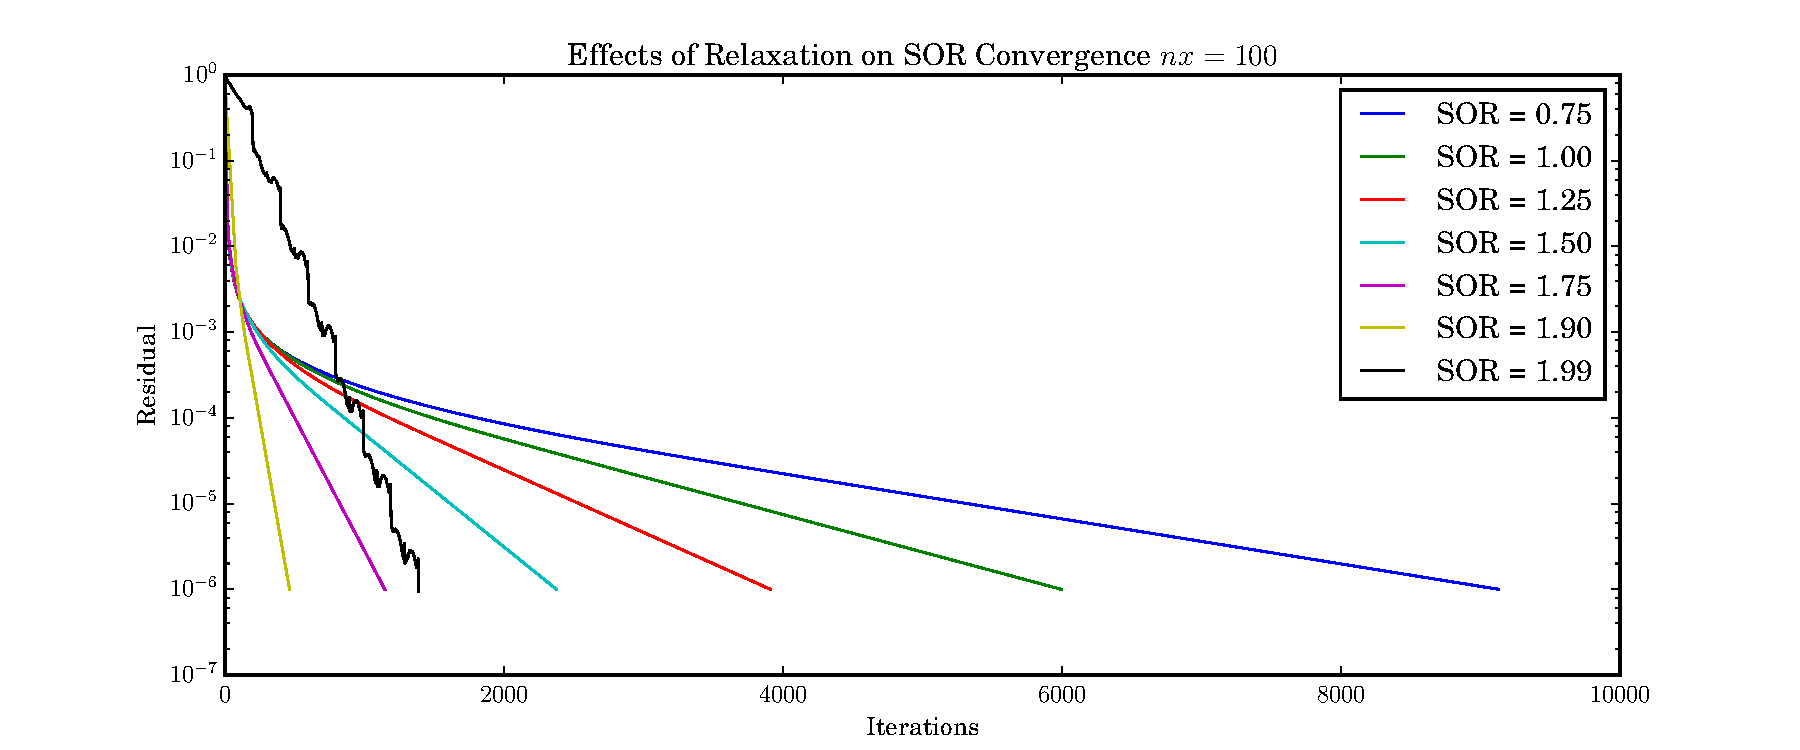
\includegraphics[width = 0.85\textwidth]{./Figures/SOR100.pdf}
    \caption{Relaxation Parameter Study $nx = 100$}
    \label{fig:sor100}
\end{figure}

\begin{figure}[!h]
    \centering
    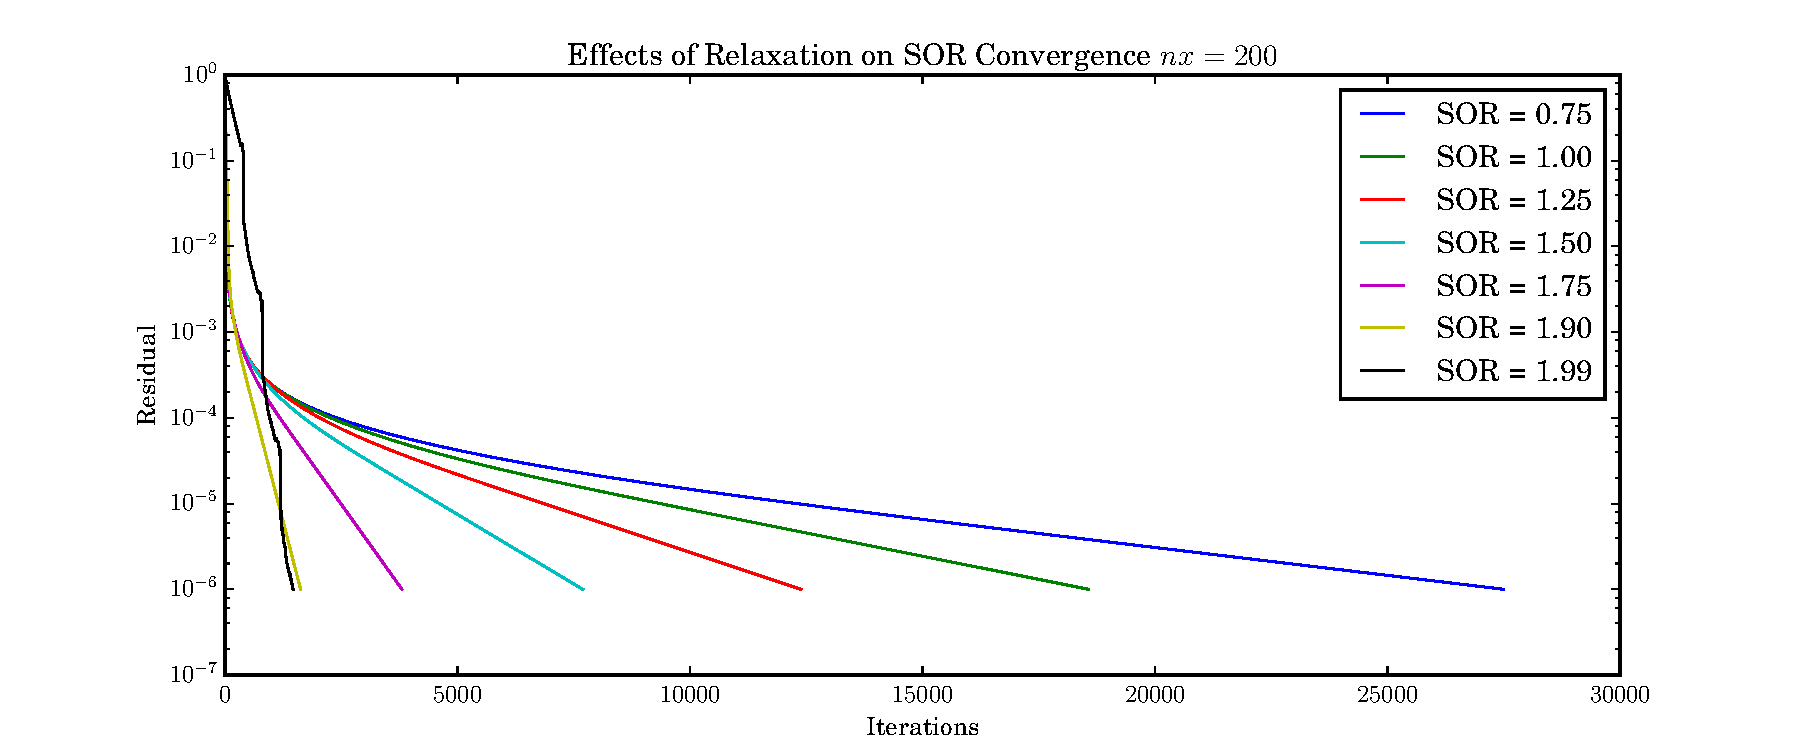
\includegraphics[width = 0.85\textwidth]{./Figures/SOR200.pdf}
    \caption{Relaxation Parameter Study $nx = 200$}
    \label{fig:sor200}
\end{figure}
\begin{figure}[!h]
    \centering
    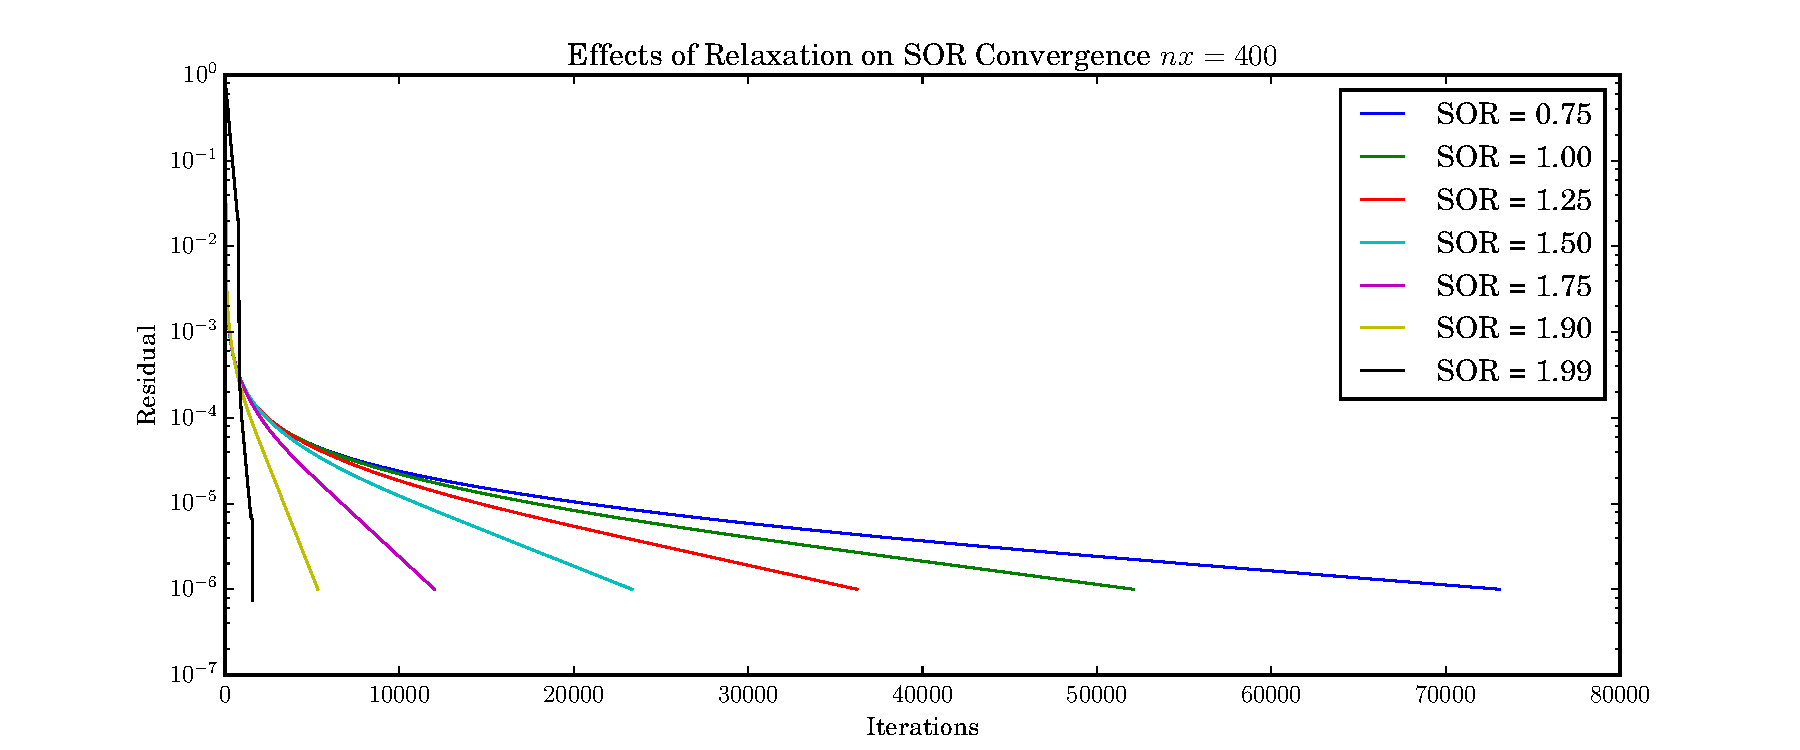
\includegraphics[width = 0.85\textwidth]{./Figures/SOR400.pdf}
    \caption{Relaxation Parameter Study $nx = 400$}
    \label{fig:sor400}
\end{figure}
\section*{Bonus}

The bonus questions are appended at the end of the document.

\section*{Codes}

Code has been written in FORTRAN. Default arithmetic operations are in double precision and optimization level -O3 unless specified otherwise.

All codes are available on my GitHub:

\url{https://github.com/dougshidong/mech539/tree/master/a2}

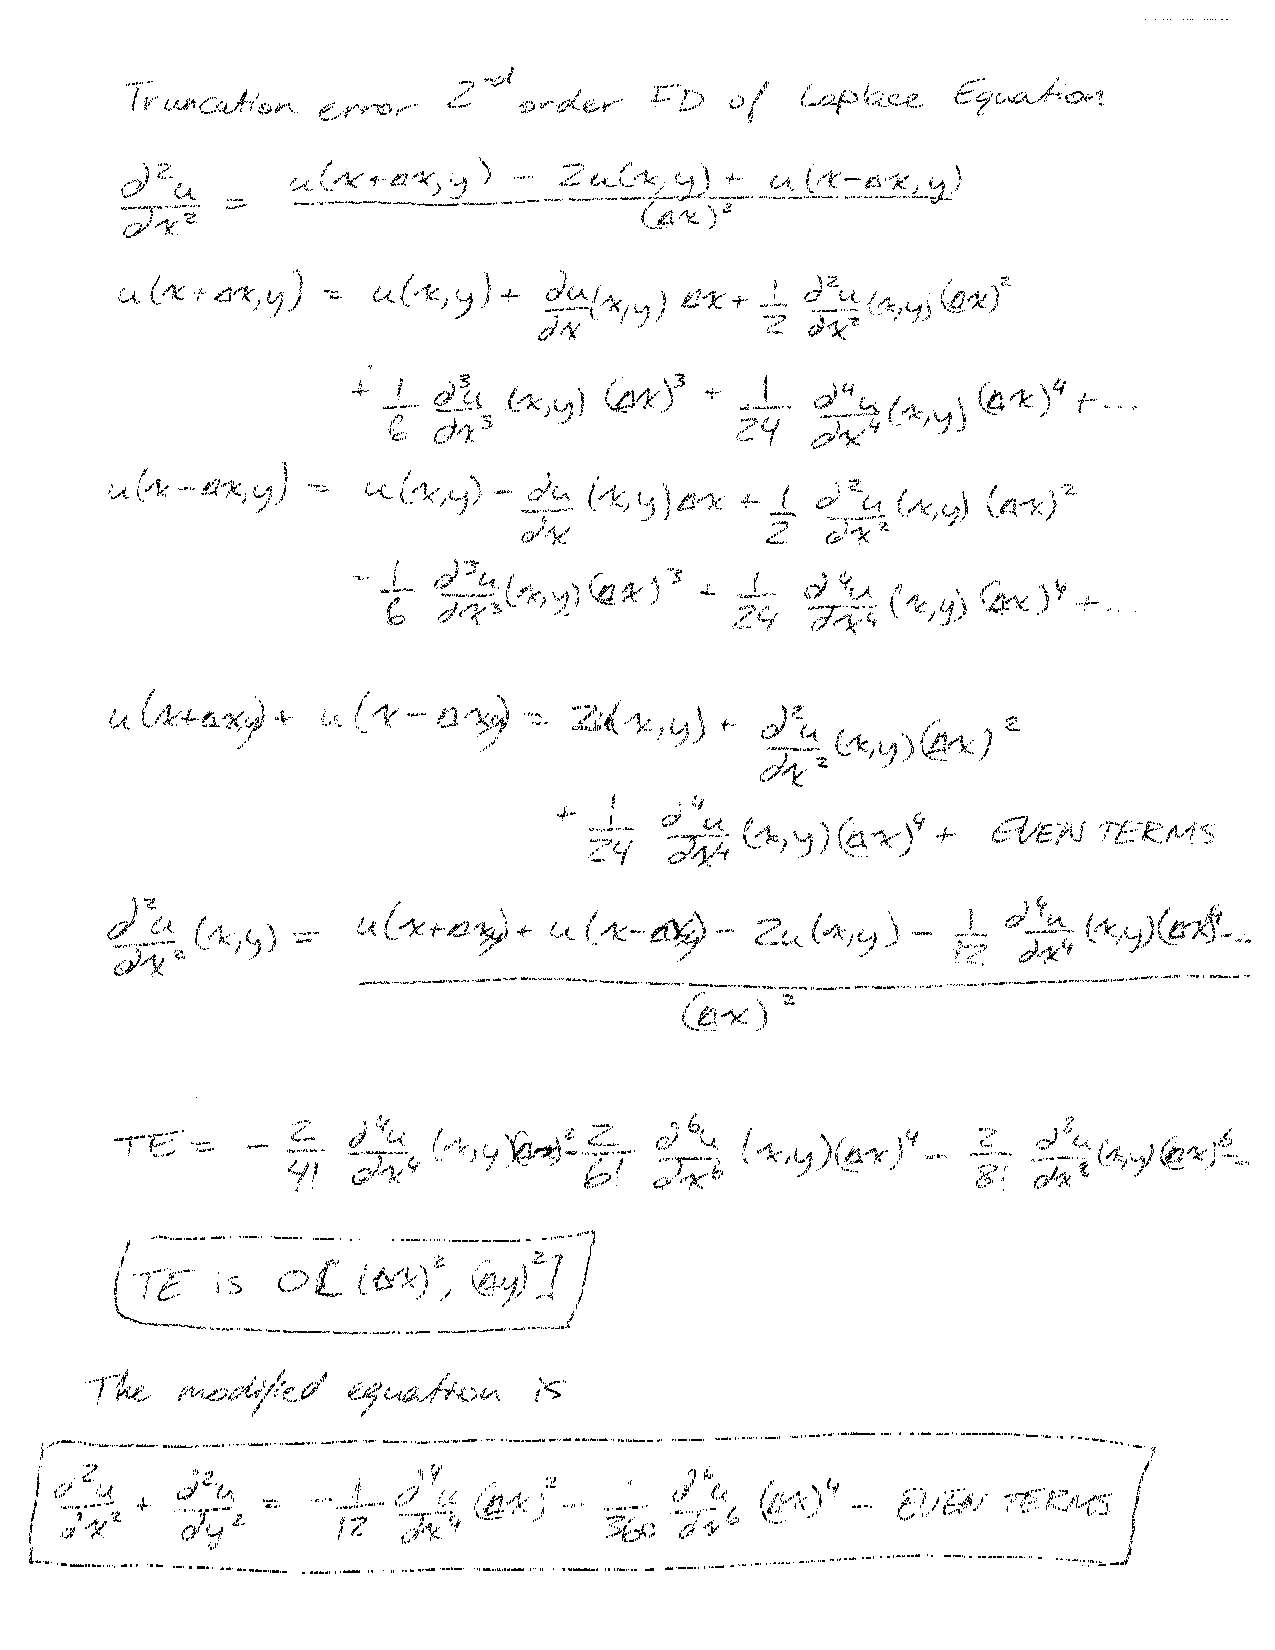
\includepdf[pages={1}]{./Figures/derivation.pdf}
\end{document}
